\documentclass[]{article}
\usepackage[T1]{fontenc} 	% codifica dei font
\usepackage[utf8]{inputenc} % lettere accentate da tastiera
\usepackage[italian]{babel} % lingua del documento
\usepackage{url} 			% per scrivere gli indirizzi Internet
\usepackage{graphicx}		% per immagini

\begin{document}

\author{Paolo Roncaglioni \and Stefano Sanitate}
\title{Progetto Ingegneria Informatica - Documento di Specifica}
\maketitle
\newpage

\begin{abstract}
Questo documento di specifica racchiude in modo organizzato tutte le ricerche, informazioni e prove che nel corso di questo progetto abbiamo raccolto, creato, analizzato. Dopo una prima parte in cui viene descritto il funzionamento generale del Bot che abbiamo pensato di progettare, si passa ai dettagli e criteri dei test che abbiamo eseguito per poter fare un deployment di una prima semplice demo del progetto descritto. La \textbf{pagina successiva} é una rappresentazione grafica di \textit{cosa} per noi é un chatBot, formalizzando i concetti raccolti e formulati per l'intero corso dello sviluppo del progetto. Si fará riferimento a questa immagine per il resto del documento. 
\end{abstract}

\tableofcontents	%generazione indice

\begin{figure}
\vspace*{-3cm} 
\centering
\includegraphics[width=2\textwidth, angle =90 ]{botofficial}
\end{figure}
\newpage

\section{Generalitá}
Il progetto é ovviamente iniziato con la delineazione dello scopo del bot, cioé che cos'avrebbe dovuto fare e a chi potrebbe essere stato utile. In un primo momento son venute fuori idee interessanti, ma magari giá presenti (e.g.\ bot orari Trenitalia) e difficilmente migliorabili.
Dopo aver quindi analizzato varie possibilitá di scelta delle funzionalitá del bot, abbiamo infine pensato di progettarne uno a tema Politecnico, che racchiuda un insieme di semplici tool allo studente (o al professore) nella gestione della propria vita universitaria. 

\subsection{Scopo}
La definizione delle caratteristiche funzionali inizia col dividerle in utenti che effettuano la propria registrazione con la coppia <Codice persona, Password> e in utenti che non lo fanno. La registrazione non é ovviamente obbligatoria, ma gli utenti loggati avranno a disposizione piú interazioni personalizzate col bot, oltre che avere tutte quelle possibili per gli utenti normali non loggati.

\paragraph{Logged Users}
\begin{enumerate}
\item \textit{Orario universitario}: richiesta orario delle lezioni, previo inserimento di tutti quei parametri che servono per identificare il corso (nome, corso di studio, sede)
\item \textit{Aule libere}: richiesta elenco aule libere, previa scelta del giorno e orario 
\item \textit{Orario aula}: richiesta elenco corsi e orari di una specifica aula (utile per controllare velocemente se l'aula davanti a te é libera)
\item \textit{Posizione aula}: restituisce semplicemente l'edificio in cui é l'aula (utile per le matricole)
\item \textit{Calendario accademico}: richiesta orario accademico, ti manda il pdf presente sul sito del Poli 
\end{enumerate}

\paragraph{UnLogged Users}
\begin{enumerate}
\item \textit{Orario universitario personalizzato}: stessa cosa della funzionalitá parte utente loggato, ma con i dati a disposizione é possibile avere maggiore accuratezza e non é richiesto l'inserimento dei dati
\item \textit{Esami}: richiesta elenco degli esami a cui ci si é iscritti
\item \textit{Informazione esami}: informazioni su esami a cui si é iscritti (i.e.\ aula, orario) 
\item \textit{Carriera didattica}: restituzione informazioni generali della propria carriera (e.g.\ media, crediti)
\item \textit{Avvisi generici}: possibilitá di settare avvisi generici con qualsiasi evento di trigger (inizialmente solo uscita voti esami con relativa votazione)
\end{enumerate}

\subsection{Personalitá}
Non sapremmo bene come prendere questa parte, poiché non ci é stato detto nulla in merito. Inizialmente di pensava di supporre che il nostro bot possa rispondere a un set di comandi predefiniti e dati da noi, non lasciando spazio all’utente per eventuali frasi complesse da interpretare. Questo approccio ci avrebbe permesso di tralasciare quasi completamente la parte sul parsing e riconoscimento degli intenti. Man mano che cominciavamo a sviluppare il nostro progetto peró ci é sembrato limitante questo approccio, poiché la vera natura del nostro progetto era di "esplorazione" di questo nuovo ambiente. Abbiamo quindi convenuto che la parte interessante sarebbe stata appunto confrontare le varie soluzioni giá presenti di NLU (natural language understanding) e rendere la conversazione col bot il piú vicino possibile a quella con un umano. Ecco quindi che si delinea l'importanza dell'utilizzo di un FrameWork che abbia queste possibilitá.

\section{Requisiti non funzionali}
Sotto questa voce vanno i requisiti e caratteristiche che impongono vincoli  allo sviluppo del bot, sotto diversi punti di vista. Per ogni problema si cercherá quindi una possibile soluzione di implementazione, che non andremo a sviluppare nella demo in quanto non riteniamo necessario in questo progetto approfondire ulteriormente.

\subsection{Prestazioni \and Price strategies}
Secondo il modello posto sopra, un bot in generale si puó rappresentare con due parti distinte, poste totalmente o in parte su un server esterno. La scelta del server influenzerá sicuramente il numero di interrogazioni che si possono fare, la velocitá di risposta e l'usabilitá in generale, a discapito del prezzo che la piattaforma di hosting ci fará pagare per avere questi servigi. Se si utilizza una soluzione "locale" in cui il proprio pc fa da server si avranno sicuramente degli svantaggi rispetto a una soluzione cloud, ma il prezzo sará nullo e le limitazioni (sulla carta) non esisterebbero. Ad ora, esplorando le varie possibili scelte, per la fase ti testing della demo é stato possibile sempre usufruire delle opzioni "free" della piattaforma di turno. Questo include sia UX che Hosting Server. Rientra in questa sezione anche la possibilitá di ridurre query rindondanti attraverso un minimo di \textit{caching}. Non é una parte da sottovalutare in quanto potrebbe risparmiarci un bel pó di interrogazioni inutili al sistema e migliorare l'efficienza generale. Si pensava quindi di usare inizialmente un'unico file di Json, che viene "guardato" dal codice ogni volta che giunge una nuova interrogazione, e aggiornato se i dati richiesti non sono presenti. É un'implementazione semplice di caching, ma per iniziare puó funzionare.  

\subsection{Privacy e persistenza}
Oltre alle informazioni pubbliche dell'utente, dobbiamo per forza aver a che fare con dati personali (e.g.\ password, codice persona ...) e riservati, che ne gli sviluppatori ne qualcuno esterno dovrebbe essere in grado di leggere. Queste informazioni doverebbero, se non vogliamo che l'utente debba sempre inserire le sue credenziali, essere tenute e criptate in qualche database esterno criptato in modo che neanche noi possano accedere al contenuto se non per interrogazione da parte del codice. Purtroppo questa problematica é una parte troppo grossa da risolvere in un progetto del genere, e potrebbe tranquillamente portarci via tutto il tempo che abbiamo pensato di dedicare al bot. Non analizzeremo dunque piú a fondo questa sezione. 

\subsection{Motore di Scraping}





\section{Flow}

\section{Ricerca del FrameWork: Bot di test}
Bot creato per testare i vari framework esistenti, aiuterá la selezione del nostro ambiente di lavoro in base a dei parametri illustrati sotto. É essenziale che sia un bot semplice (per non perdere troppo tempo con lo sviluppo, essendo di test), ma con funzionalitá che siano correlate alla costruzione del nostro progetto in specifica. Pertanto ecco le regole che pensiamo debba soddisfare.

\subsection{Requisiti}
\begin{itemize}
\item Interazione basilari con un’API web (bisogna che sia semplice e facile da usare)
\item Riconoscimento domande al bot, piú domande poste in modo diverso devono essere riconosciute (e.g. com'è il tempo domani Milano? = che tempo fa domani a milano?)
\item Riconoscimento semplici entitá date dall’utente (e.g. luogo, ora, data, nome, ..)
\end{itemize}

\subsection{Parametri di valutazione}
Questi rappresentano i parametri che useremo per valutare il framework che testeremo. Essi comprendono sia i componenti di valutazione della costruzione del bot, che quelli piú generali della piattaforma che stiamo usando. La valutazione è a nostra discrezione, ovviamente seguita da una minima descrizione delle procedure svolte.

\paragraph{Bot}
\begin{itemize}
\item \textit{Facilitá di progettazione}: Quante conoscenze e approfondimenti sono necessari per creare il bot
\item \textit{Tempo di implementazione}: Quanto tempo impieghiamo a creare il bot finito funzionante
\item \textit{Profondità}: L’insieme di strumenti aggiuntivi che ci sono forniti dall’ambiente di lavoro (training, analisi, ..) che permettono uno sviluppo piú approfondito del bot
\item \textit{Persistenza della memoria}: possibilitá (e facilitá) di memorizzare certi dati dell’utente per un certo periodo di tempo
\end{itemize}

\paragraph{FrameWork}
\begin{itemize}
\item \textit{Pricing strategies}: Prezzo e fornitori
\item \textit{Piattaforme}: Su quali piattaforme di chat (telegram, slack, ..) posso fare il deployment
\item \textit{Disponibilitá di SDK}: utili allo sviluppo, non enormemente influenti in questo test
\end{itemize}

\subsection{Descrizione bot}
Il tipo di bot(test) che alla fine abbiamo scelto di portare avanti è una semplice implementazione di chatbot “Che tempo fa?”, cioè data una localitá (milano, monza, ..) e un giorno (oggi, domani, 31/12/2017, ..) restituisce il tempo meteo della localitá scelta nella data scelta. Questo dovrebbe permetterci di esplorare tutti i parametri sopra descritti.
La scelta è ricaduta su questo tipo di bot soprattutto grazie alla disponibilitá di una documentazione passo-passo da parte del frameWork DialogFlow dell'implementazione del bot descritto sopra (presente nella repository di github di riferimento).

\subsection{Deployment description}
In questa parte andiamo a descrivere la nostra esperienza con le 8 (su 25-30 di base) piattaforme individuate tramite ricerca e con supporto di questo,  questo e questo (valido anche se datato) documento. Abbiamo escluso tutte quelle applicazioni per il quale non è stato possibile reperire il prezzo o che proponevano solo dei Trial o Demo (tipicamente pensate per aziende) o quelle che pensiamo non abbiano gli elementi base per poter servire al progetto.
Per l’hosting e il deployment del codice (funzione weatherWebhook) che è servito da base per l’interazione con API esterne, abbiamo usato la piattaforma Google Cloud Project, usufruendo del servizio gratis per 1 anno. Per quanto riguarda l’API key, abbiamo sfruttato quella del famoso sito \url{https://developer.worldweatheronline.com}, che permette di avere la premium key per un periodo di trial di 60 giorni (500 calls per minuto). Una parte su cui abbiamo avuto difficoltá inizialmente è stata la configurazione del servizio di google, ma una volta messo in piedi la struttura della generazione delle risposte dovrebbe essere possibile sfruttare questo script su tutte le piattaforme di testing.

\subsubsection{DialogFlow} 
\paragraph{Implementazione}
La piattaforma permette di creare degli “agent”, contenitori che servono a raccogliere i vari pezzi di riconoscimento delle risposte (“intent”). All’interno di un agent possiamo creare piú intent, cosicché  la struttura finale risultante puó risultare anche abbastanza complessa. Piú intent possono essere concatenati creando un contesto. All’interno di un intent possiamo creare un processo di riconoscimento della domanda data dall’utente, preimpostando una risposta (testuale e non). All’interno del set di domande che l’utente puó scrivere, si possono settare dei “parameter” (gestione quasi automatica del parsing, possiamo comunque scegliere alcuni aspetti del json) che verrebbero quindi usati per la generazione delle risposte. Il riempimento dei parametri puó essere settato per essere preso all’esterno della piattaforma (usando un webHook) in modo molto semplice, inviando e ricevendo sempre un file in formato json. Detto questo è quindi bastato settare un paio di domande e risposte negli intent che abbiamo creato, inserire il giusto indirizzo di webhook e il bot è stato creato e testato su console e sul servizio di chat Telegram.

\begin{figure}
\makebox[\textwidth][c]{%
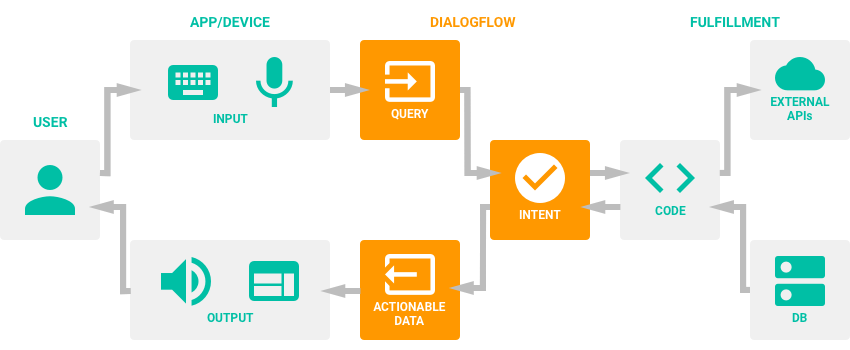
\includegraphics[width=1.2\textwidth]{dialogflow}
}
\caption{ \footnotesize{DialogFlow in breve}}
\end{figure}

\paragraph{Valutazione}
\begin{itemize}
\item \textit{Facilitá di progettazione}: \textbf{9} \\ molto semplice e intuitivo, senza bisogno di metter mano a codice

\item \textit{Tempo di implementazione}: \textbf{9} \\ 2 ore (se non contiamo il setting di google cloud)  

\item \textit{Profondità}: \textbf{8} \\  permette di creare facilmente contesti di riconoscimento, presenza di azioni di trigger ed eventi facilmente configurabili, sezione “Training” attivabile, riconoscimente delle domande e parametri non prima specificati
\item \textit{Persistenza della memoria}: \textbf{7} \\ permette di tenere traccia di parametri (settando una lifespan) da poter riusare nel giusto contesto, non abbiamo svolto ulteriori ricerche
\item \textit{Pricing strategies}: \textbf{9} \\ piattaforma completamente gratuita per la progettazione e per il deployment finchè non si raggiungono un certo numero di richieste al minuto, poi hai l’opzione di aumentare il proprio piano

\item \textit{Piattaforme}: \textbf{9} \\ vasta estensione, comprende buona parte dei servizi piú usati ad oggi di chat (messenger, telegram, twitter, ..) e non (slack, google assistant, cortana,..) 
\item \textit{Disponibilitá di SDK}: \textbf{10} \\  presente buona parte dei linguaggi di programmazione piú usati o utili
\end{itemize}

\paragraph{Commento personale}
DialogFlow (ex API.ai) é un ottimo candidato al framework che useremo nel nostro progetto. Semplice e intuitivo, permette di creare semplici o complessi bot se usato nel pieno potenziale, senza perder troppo tempo con il parsing di risposte/domande. Ha molte funzioni interessanti che non abbiamo approfondito, ma che risulterebbero utili al nostro sviluppo. 

\subsubsection{FlowXo}
\paragraph{Implementazione}
FlowXo è il primo servizio nel quale per prima viene chiesta la piattaforma per la quale sviluppare il bot. Ho scelto Telegram: il sito si appoggia a @BotFather per creare e autenticare il proprio bot. Ad un proprio bot è possibile associare un flow, nel quale è possibile assegnare una serie di azioni (tra cui una richiesta http, nel nostro caso).
\paragraph{Valutazione}
\begin{itemize}
\item \textit{Facilitá di progettazione}: \textbf{9} \\
\item \textit{Tempo di implementazione}: \textbf{9} \\
\item \textit{Profondità}: \textbf{9} \\
\item \textit{Persistenza della memoria}: \textbf{9} \\
\item \textit{Pricing strategies}: \textbf{9} \\
\item \textit{Piattaforme}: \textbf{9} \\
\item \textit{Disponibilitá di SDK}: \textbf{9} \\
\end{itemize}
\paragraph{Commento personale}

\subsubsection{PandoraBots}
\paragraph{Implementazione}
\paragraph{Valutazione}
\begin{itemize}
\item \textit{Facilitá di progettazione}: \textbf{9} \\
\item \textit{Tempo di implementazione}: \textbf{9} \\
\item \textit{Profondità}: \textbf{9} \\
\item \textit{Persistenza della memoria}: \textbf{9} \\
\item \textit{Pricing strategies}: \textbf{9} \\
\item \textit{Piattaforme}: \textbf{9} \\
\item \textit{Disponibilitá di SDK}: \textbf{9} \\
\end{itemize}
\paragraph{Commento personale}

\subsubsection{GupShup.io}
\paragraph{Implementazione}
\paragraph{Valutazione}
\begin{itemize}
\item \textit{Facilitá di progettazione}: \textbf{9} \\
\item \textit{Tempo di implementazione}: \textbf{9} \\
\item \textit{Profondità}: \textbf{9} \\
\item \textit{Persistenza della memoria}: \textbf{9} \\
\item \textit{Pricing strategies}: \textbf{9} \\
\item \textit{Piattaforme}: \textbf{9} \\
\item \textit{Disponibilitá di SDK}: \textbf{9} \\
\end{itemize}
\paragraph{Commento personale}

\subsubsection{Microsoft Bot Framework}
\paragraph{Implementazione}
\paragraph{Valutazione}
\begin{itemize}
\item \textit{Facilitá di progettazione}: \textbf{9} \\
\item \textit{Tempo di implementazione}: \textbf{9} \\
\item \textit{Profondità}: \textbf{9} \\
\item \textit{Persistenza della memoria}: \textbf{9} \\
\item \textit{Pricing strategies}: \textbf{9} \\
\item \textit{Piattaforme}: \textbf{9} \\
\item \textit{Disponibilitá di SDK}: \textbf{9} \\
\end{itemize}
\paragraph{Commento personale}

\subsubsection{Wit.ai}
Dopo aver consultato la guida per iniziare e aver cominciato a creare qualcosa, mi son reso conto che mancavano delle funzioni significative. Ho appreso che facebook sta chiudendo la piattaforma in modo da integrare il “natural language processing (NPL)  tools into Messenger Platform 2.1”

\subsubsection{ChatFuel}
\paragraph{Implementazione}
Nel servizio è presente solo la possibilitá di maneggiare la struttura del bot solo tramite GUI. Interfaccia molto semplice, presenza di “Blocks” che permettono di modellare l’automatizzazione di azioni (presa input, richieste http, stampa video,..) e “Groups” nella quale racchiudere a piacimento questi blocks. I suddetti blocchi possono essere concatenati in sequenze a seconda del bisogno, ed esistono strutture che permettono di maneggiare queste transizioni (da blocco a blocco - da sequenza a sequenza) in modo quasi intuitivo e completo. Questi blocchi possono avere una vasta gamma di eventi di trigger, ma principalmente vengono richiamati dalla sezione ”””””AI””””” che permette di inserire delle frasi (con “riconoscimento del contesto”)  ed eseguire di conseguenza un dato blocco. Dopo aver capito i funzionamenti base della piattaforma dunque è bastato creare un singolo blocco con la giusta presa di input dall’utente e una richiesta http per creare il bot desiderato. Da notare l’impossibilitá di testare il bot su una qualche console ma solo direttamente sulla propria pagina facebook (alla quale si deve per forza collegare il bot). Per completezza del documento, in questa piattaforma è stato necessario ri-adattare il codice in Node.js descritto all’inizio di questo testo, in modo che ricevesse del codice Json in entrata e uscita leggermente diversi, come scritto sulla repository di github.

\begin{figure}
\makebox[\textwidth][c]{%
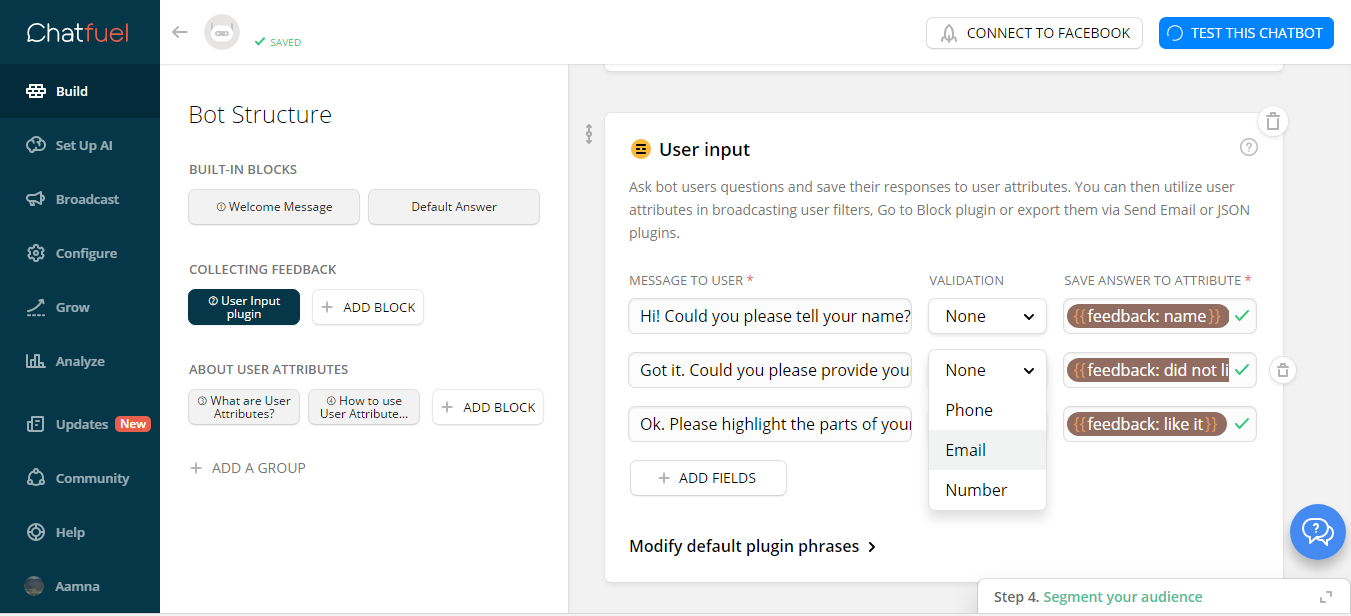
\includegraphics[width=1.2\textwidth]{chatfuel}
}
\caption{ \footnotesize{Panoramica della piattaforma (user input plugin)}}
\end{figure}

\paragraph{Valutazione}
\begin{itemize}
\item \textit{Facilitá di progettazione}: \textbf{8} \\ A parte la difficoltá nel trovare il giusto formato Json, l’intera piattaforma è molto intuitiva (presente solo interfaccia grafica)
\item \textit{Tempo di implementazione}: \textbf{9} \\ 2,5 ore, senza contare lo sviluppo del motore su Google Cloud (giá fatto per altri framework)
\item \textit{Profondità}: \textbf{6} \\ Da un lato è molto limitante (ad esempio, non è possibile fare un parsing di una frase in modo da ottenere specifici parametri, ma si deve dar la possibilitá all’utente di inserirli volta per volta), dall’altro è interessante la possibilitá di usare Plugin modulabili a piacimento (sia interni che esterni), anche se preimpostati. Presenza di diversi tool di analisi e broadcast facile
\item \textit{Persistenza della memoria}: \textbf{6} \\  All’interno di un blocco è possibile tenere traccia delle variabili o parametri dell’utente
\item \textit{Pricing strategies}: \textbf{8} \\  piattaforma gratuita, ma previa creazione di pagina facebook. Possibilitá di sottoscrivere abbonamento per un servizio migliore
\item \textit{Piattaforme}: \textbf{3} \\ Implementato solo in facebook
\item \textit{Disponibilitá di SDK}: \textbf{9} \\ n/a
\end{itemize}
\paragraph{Commento personale}

\subsubsection{kitt.ai}
\paragraph{Implementazione}
\paragraph{Valutazione}
\begin{itemize}
\item \textit{Facilitá di progettazione}: \textbf{9} \\
\item \textit{Tempo di implementazione}: \textbf{9} \\
\item \textit{Profondità}: \textbf{9} \\
\item \textit{Persistenza della memoria}: \textbf{9} \\
\item \textit{Pricing strategies}: \textbf{9} \\
\item \textit{Piattaforme}: \textbf{9} \\
\item \textit{Disponibilitá di SDK}: \textbf{9} \\
\end{itemize}
\paragraph{Commento personale}

\subsection{Commenti Finali e decisione}


\section{Costruzione bot di Demo}
\subsection{ServerSide}
\subsection{UX (DialogFlow)}
\subsection{Limitazioni}

\section{Futuri Sviluppi}

% Bibliografia
\begin{thebibliography}{9}
\url{https://dialogflow.com} \\
\url{https://github.com/Roncax/PolimiChatBot} \\
\url{https://dialogflow.com} \\
\url{https://dialogflow.com} \\
\url{https://dialogflow.com} \\
\url{https://dialogflow.com} \\
bibliografia, software usati, github repo.
\end{thebibliography}

\end{document}
